\documentclass[11pt,a4paper]{article}

\usepackage[margin=2.2cm]{geometry}
\usepackage[T1]{fontenc}
\usepackage{lmodern}
\usepackage{booktabs}
\usepackage{array}
\usepackage{graphicx}
\usepackage{float}
\usepackage{caption}
\usepackage{tikz}
\usetikzlibrary{positioning,arrows.meta}
\usepackage[hidelinks]{hyperref}

\setlength{\parskip}{4pt}
\setlength{\parindent}{0pt}
\captionsetup{font=small}
\renewcommand{\arraystretch}{1.25}
\newcolumntype{L}[1]{>{\raggedright\arraybackslash}p{#1}}
\setlength{\tabcolsep}{4.5pt}
\newcommand{\hd}[1]{\begin{tabular}[b]{@{}c@{}}#1\end{tabular}}
\newcommand{\rowline}{\specialrule{0.2pt}{3pt}{3pt}}

\title{DPDP-Audit: Mid-Submission Report\\[2pt]
\large Checking app privacy policies against app behaviour under India's DPDP Act}
\author{Anurag Kaushal\\2025202013 \and Ishaan Giri\\2025201091 \and Naveen Mishra\\2025201084
\and Nikhil Patidar\\2025201081}
\date{30 October 2026\\[2pt]
Code and data: \url{https://github.com/Anurag-1205/DPDP-Audit}}

\begin{document}
\maketitle

\section{Summary}

An app's privacy policy says what personal data it collects, why, and who receives it. The app's
code and its third-party SDKs may do something else. We call such a difference a \emph{compliance
gap}. We study five kinds of gap under India's Digital Personal Data Protection (DPDP) Act,
2023~\cite{dpdpact,dpdprules}: undisclosed collection, undisclosed sharing, purpose mismatch,
retention mismatch and children's data.

So far we have:
\begin{itemize}
  \item built a benchmark of 102 app and policy cases from the OPP-115 corpus~\cite{opp115}, whose
        answers come from fixed rules over expert annotations (no LLM in the ground truth), and a
        140-case \emph{vagueness ladder};
  \item run two published checkers (PoliCheck~\cite{policheck} and PoliGraph~\cite{poligraph}),
        three single-prompt LLM baselines, and three baselines built from our pipeline's own parts;
  \item built DPDP-Audit, an evidence-based review pipeline, in two versions (v1 and v2), with a
        clause tagger fine-tuned with QLoRA~\cite{qlora};
  \item had two team members check the ladder and a sample of the answer keys by hand.
\end{itemize}

\textbf{Main result.} Our final system (v2 with the fine-tuned tagger) reaches an F1 of 0.705 with a
false-alarm rate of 0.265 on compliant apps (Figure~\ref{fig:main}). The best single-prompt baseline,
Gemini 3 Flash given the same prompt as our single-prompt baseline B2, reaches F1 0.421 but raises an
alarm on 97\% of compliant apps. The published tools reach F1 0.149 (PoliCheck) and 0.166
(PoliGraph). All of v2's F1 gains over the baselines are statistically significant on every seed. It
also has significantly fewer false alarms than every baseline except the one-review-call baseline B5,
which is about as safe.

\textbf{Where the gain comes from.} Baselines built from the pipeline's own parts show what each
layer adds. Rules alone (our tagger and the finder, no LLM) already reach F1 0.524 but raise an
alarm on 91\% of compliant apps. One review call that quotes the evidence first, followed by our
decision rules and verifier, reaches F1 0.557 with 25\% false alarms. The full pipeline adds a
further +0.13 to +0.16 F1 on every seed.

\textbf{What did not work.} The first version (v1) does not beat the single-prompt baseline on F1.
The evidence verifier costs more recall than we allowed, and the reviewer agents never used their
tools. Purpose findings are v2's largest source of false findings: almost every purpose gap it
reports is wrong (Finding~\ref{find:purpose}). On ladder rungs where the disclosure was deleted, the
pipeline is right only 14\% of the time, because it reads unrelated or generic wording as a vague
disclosure. Section~\ref{sec:hyp} lists every hypothesis with its verdict.

\begin{figure}[H]
\centering
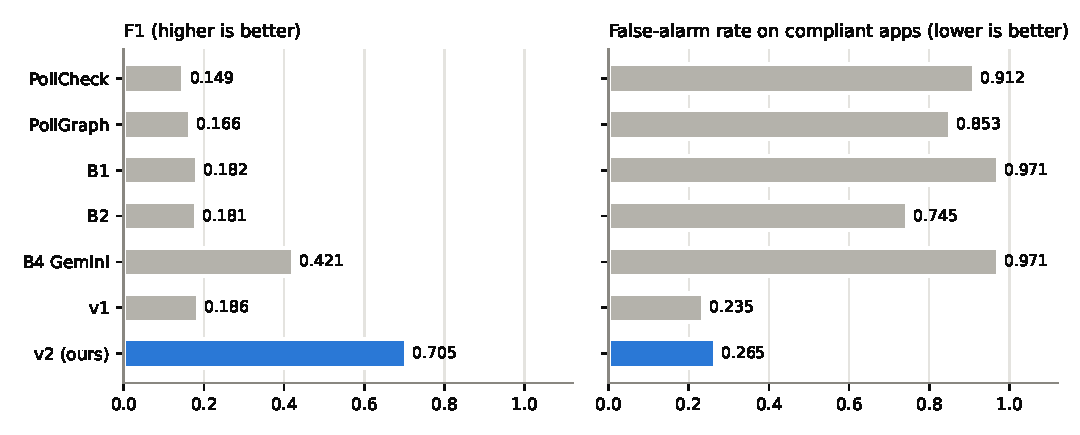
\includegraphics[width=\textwidth]{figures/main_results.pdf}
\caption{F1 and false-alarm rate on the main benchmark (mean over seeds). Only v2 is both accurate
and safe. The stronger model B4 and the rules-only R0 find many gaps but alarm on almost every
compliant app; B5 is safe but finds fewer gaps.}
\label{fig:main}
\end{figure}

\section{Research questions and hypotheses}

\begin{itemize}
  \item \textbf{RQ1 (main).} Does a multi-stage, evidence-based review pipeline grounded in the DPDP
        Act find more gaps than the published flow-to-policy tools and than single-prompt review by
        the same model, with fewer false alarms?
  \item \textbf{RQ2 (wording).} When only one sentence of a policy changes (clear, explicit denial,
        vague, deleted), how does each system's verdict on the same data flow change?
  \item \textbf{RQ3 (review cost).} How much human review does each system need before the rest of
        its output reaches 95\% accuracy? (Stage 4.)
  \item \textbf{RQ4 (reading).} How much of the remaining error comes from reading the policy rather
        than from legal reasoning, and how close does a fine-tuned 3B tagger come to
        PrivBERT~\cite{privaseer}?
\end{itemize}

Hypotheses: \textbf{H1} our system beats PoliCheck and PoliGraph on collection and sharing gaps;
\textbf{H2} it beats the single-prompt baselines B1 and B2, most on vague and omission gaps;
\textbf{H3} the verifier lowers false alarms while losing at most 5 points of recall; \textbf{H4}
every system is less accurate on vague than on explicit rungs; \textbf{H5} our system needs less
human review than B2 for 95\% accuracy; \textbf{H6} the fine-tuned tagger beats a prompted 3B
tagger, comes within 5 points of PrivBERT, and closes half the gap to a perfect (gold) tagger.
\textbf{Falsifiable claim:} our system beats both tools on their gap types and B2 on the full
benchmark, in both F1 and false-alarm rate.

\textbf{Related work.} PoliCheck~\cite{policheck} labels each (data type, recipient) flow of an app
as clearly, vaguely, ambiguously or incorrectly disclosed, or omitted, using the statements
PolicyLint~\cite{policylint} extracts and fixed ontologies. PoliGraph~\cite{poligraph} turns a policy
into a knowledge graph, and PurPliance~\cite{purpliance} also compares stated purposes. Recent work
applies LLMs to policy and code consistency~\cite{mao2025} and to GDPR checks for Android
apps~\cite{alecci2025}, and compares LLMs with the classic tools~\cite{aryal2026}. We differ in three
ways: we ground every finding in a quoted policy sentence and a DPDP section, with rules (not the
model) deciding the gap; we evaluate on a controlled benchmark whose answers come from scripts, not
from people or an LLM; and we compare the published tools, single-prompt LLMs and our pipeline
head to head on the same cases.

\section{Datasets and benchmark}

\begin{table}[H]
\centering
\small
\begin{tabular}{L{3.6cm}L{5.2cm}L{5.4cm}}
\toprule
Dataset & What it is & How we use it \\
\midrule
\textbf{OPP-115~\cite{opp115}} & 115 website privacy policies with paragraph-level expert
annotations of data practices & Split 80 training / 35 held out (seed 13). Held-out policies build
the benchmark and ladder; training policies give the tagger data (2,426 paragraphs) and the dev
splits \\ \rowline
\textbf{DPDP Act 2023 and Rules 2025~\cite{dpdpact,dpdprules}} & The official text, split into 153
citable units & Retrieval for the reviewers, and checking that every cited section exists \\ \rowline
\textbf{SDK table (ours)} & 20 common Android SDKs with vendor, category and network domains &
Naming recipients and recognising ad and tracking SDKs \\ \rowline
\textbf{PoliCheck released flows~\cite{policheck}} & 186,578 real network flows from 22,422 Android
apps, with policy links & Stage 4 real-flow sample, with policies archived in 2019 \\
\bottomrule
\end{tabular}
\caption{Datasets used. All are public or built by us; no paid data.}
\end{table}

From these we build three evaluation sets:

\begin{table}[H]
\centering
\small
\begin{tabular}{L{2.6cm}L{5.4cm}L{6.2cm}}
\toprule
Set & Size & Answer source and status \\
\midrule
\textbf{Main} & 102 cases (34 compliant controls, 68 variants), 118 gold gaps, 433 data flows &
Fixed rules over expert OPP-115 annotations. A hand check of 87 flows found the key wrong on
9 flows (10.3\%). \\ \rowline
\textbf{Vagueness ladder} & 140 cases: 35 ladders of 4 rungs (clear, explicit, vague, deleted) &
One templated sentence changes per rung. Checked by two members; 110 rungs accepted. \\ \rowline
\textbf{Dev splits} & 33 + 69 cases from 34 training policies & Same rules. Used only to develop
the pipeline, never for evaluation. \\
\bottomrule
\end{tabular}
\caption{Benchmarks. The 35 OPP-115 policies held out from training (80/35 split, seed 13) give the
ladder; the main benchmark uses 34 of them (3 cases each), because one has no clearly disclosed
flow for a control.}
\end{table}

A case is not a working app. It is a policy plus three small files that describe what an app does:
a build file listing its SDKs, an Android manifest with its permissions (and whether it is
child-directed), and a list of data flows (data type, recipient, purpose, retention).

\textbf{How cases are made.} For each held-out policy, the generator first indexes what the
annotations say: which data types are collected and why, which are shared and with whom, which
are explicitly not collected or shared, retention promises and children statements. It then builds
one \emph{control}: up to 3 collection flows and up to 2 SDK sharing flows that the policy clearly
covers, so the rules give it zero findings. Two \emph{variants} copy the control and plant 1 or 2
flows that the policy does not cover, choosing the least-used (gap type, level) cell each time so
rare cells fill first. Every flow is then checked by the rules, not only the planted one. The
generator is deterministic: running it again gives byte-identical files.

\begin{table}[H]
\centering
\small
\begin{tabular}{L{2.5cm}L{3.3cm}L{3.5cm}L{2.7cm}L{2.0cm}}
\toprule
Gap type & Explicit & Vague & Omission & DPDP \\
\midrule
\textbf{Undisclosed collection} & policy says it does not collect the type & only generic data is
collected & nothing mentions it & Sec. 5(1), 6(1) \\ \rowline
\textbf{Undisclosed sharing} & policy says it does not share the type, and no sharing of it is
stated & shared, but not with this recipient for a stated purpose (or only generic data is
shared) & nothing mentions it & Sec. 5(1), 6(1) \\ \rowline
\textbf{Purpose mismatch} & & the app's purpose is not stated, and the stated purposes include an
unspecified one & stated purposes exclude the app's purpose & Sec. 5(1), 6(1) \\ \rowline
\textbf{Retention mismatch} & policy gives a period or limit & retention mentioned without a
period & no retention statement & Sec. 8(7) \\ \rowline
\textbf{Children's data} & policy has a children statement & & no children statement &
Sec. 9(3) \\
\bottomrule
\end{tabular}
\caption{Gap types and levels as the answer-key rules define them, with the DPDP sections a
finding must cite. A level's label is \emph{incorrect} (explicit), \emph{vague} or
\emph{omitted}. Purpose is checked only when the flow itself is clearly disclosed, so a flow never
has both a notice gap and a purpose gap.}
\end{table}

\section{Systems}

\begin{table}[H]
\centering
\small
\begin{tabular}{lL{7.6cm}l}
\toprule
ID & System & Model \\
\midrule
\textbf{S1} & PoliCheck (authors' code)~\cite{policheck} & rule-based NLP \\ \rowline
\textbf{S2} & PoliGraph (authors' released NLP version)~\cite{poligraph} & rule-based NLP \\ \rowline
\textbf{B1} & One prompt with the raw policy and app files & Qwen2.5-7B \\ \rowline
\textbf{B2} & One prompt with exactly the inputs our pipeline gets & Qwen2.5-7B \\ \rowline
\textbf{B4} & B2's prompt given to a much stronger model & Gemini 3 Flash \\ \rowline
\textbf{v1} & DPDP-Audit as frozen before evaluation & Qwen2.5 3B tagger, 7B reviewers \\ \rowline
\textbf{v2} & DPDP-Audit with fixes chosen on the dev splits only (Section~\ref{sec:v2}) &
same \\ \rowline
\textbf{A1 to A5} & Ablations: verifier off, no retrieval, one generalist reviewer, oracle
tagger & same \\ \rowline
\textbf{R0} & Rules only: our tagger and the finder, every candidate reported & no LLM \\ \rowline
\textbf{B5} & One review call over the whole policy, evidence first, then v2's rules and
verifier & Qwen2.5-7B \\ \rowline
\textbf{B1, B2, B4 sc} & Self-consistency~\cite{selfconsistency}: the majority label over the
three seeds & as the system \\
\bottomrule
\end{tabular}
\caption{End-to-end systems. B1, B2, B4, B5, v1 and v2 run with 3 seeds (0, 1, 2); the v2
ablations also run with 3 seeds and the v1 ablations with seed 0 only; the tools and R0 are
deterministic and run once; each self-consistency row is one combined output of the three seeds.
R0, B5 and the self-consistency rows were added on 30 October (Section~\ref{sec:parts}).}
\end{table}

\textbf{Tagger-level systems} (Section~\ref{sec:tagger}) read policy paragraphs only: S3 PrivBERT, a
fine-tuned category classifier~\cite{privaseer}; B3, a prompted Qwen2.5-3B that predicts categories
only; S4, the statement extraction of PolicyLint~\cite{policylint} and PoliGraph; and our QLoRA
tagger.

\textbf{Models and settings.} The LLM systems use Qwen2.5-7B-Instruct-AWQ~\cite{qwen25} served with
vLLM~\cite{vllm} on two Kaggle T4 GPUs; the tagger is Qwen2.5-3B-Instruct; B4 uses
\texttt{gemini-3-flash-preview} through its API. Reviewer and baseline calls use temperature 0.7
with seeds 0, 1 and 2; the verifier and the tagger use temperature 0.

\begin{figure}[H]
\centering
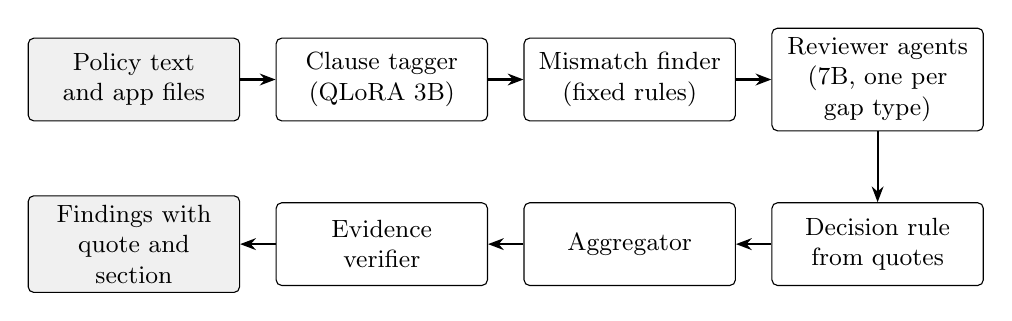
\begin{tikzpicture}[
  box/.style={draw, rounded corners=2pt, align=center, font=\small,
              minimum height=1.05cm, text width=2.45cm, fill=white},
  io/.style={box, fill=gray!12},
  arr/.style={-{Stealth[length=2mm]}, thick},
  node distance=0.45cm]
\node[io] (in) {Policy text\\and app files};
\node[box, right=of in] (tag) {Clause tagger\\(QLoRA 3B)};
\node[box, right=of tag] (find) {Mismatch finder\\(fixed rules)};
\node[box, right=of find] (rev) {Reviewer agents\\(7B, one per\\gap type)};
\node[box, below=0.9cm of rev] (rule) {Decision rule\\from quotes};
\node[box, left=of rule] (agg) {Aggregator};
\node[box, left=of agg] (ver) {Evidence\\verifier};
\node[io, left=of ver] (out) {Findings with\\quote and section};
\draw[arr] (in) -- (tag);
\draw[arr] (tag) -- (find);
\draw[arr] (find) -- (rev);
\draw[arr] (rev) -- (rule);
\draw[arr] (rule) -- (agg);
\draw[arr] (agg) -- (ver);
\draw[arr] (ver) -- (out);
\end{tikzpicture}
\caption{The DPDP-Audit pipeline. The tagger turns each policy paragraph into structured claims.
The finder proposes every flow those claims do not clearly cover. A reviewer copies the policy
sentences that disclose, deny or only vaguely cover the flow. A fixed rule turns the verified
quotes into a gap and its level. The verifier drops findings with a wrong quote or DPDP section and
sends doubtful ones to human review.}
\end{figure}

\subsection{A worked example}

Case \texttt{1050\_v1} uses a car-finance company's policy. The app is child-directed and sends
\emph{IP address and device IDs} to Google AdMob for advertising (flow f5). We follow this flow;
the case's third finding is noted at the end.
\begin{enumerate}
  \item \textbf{Finder.} The tagger's claims cover this sharing only through unnamed recipients and
        generic data, so the finder proposes an undisclosed-sharing candidate (suggested level
        vague). Because the app is child-directed and AdMob is an advertising SDK, it also proposes
        a children's-data candidate.
  \item \textbf{Reviewer.} The notice reviewer quotes the generic sentence ``Information about you
        to nonaffiliated third parties as permitted or required by law (for example, information
        provided to credit reporting agencies or in response to a subpoena).'' It also offers, as a
        denial, a sentence about a separate financial privacy policy.
  \item \textbf{Decision rule.} Both quotes are found word for word in the policy. The ``denial''
        does not name the data type, so the rule ignores it. The generic quote names neither the
        data type nor Google, so the level is \emph{vague}. The children's reviewer finds no
        children statement, so that gap is an \emph{omission}.
  \item \textbf{Verifier and output.} The quotes and sections are valid, so v2 reports two findings
        for this flow: undisclosed sharing (vague, citing Sec. 5(1)) and children's data (omission,
        citing Sec. 9(3)). Both match the answer key.
\end{enumerate}
v2 also reports a third finding on this case (seed 0): a purpose gap on flow f4, where the app
collects demographic data for advertising (vague, citing Sec. 5(1)). It matches the answer key and
is v2's only correct purpose finding on seed 0. Its quoted sentence, however, is about cookies being
anonymous, not about purposes, which shows why purpose findings are v2's weakest part
(Finding~\ref{find:purpose}).

\section{Results on the main benchmark}

Table~\ref{tab:main} gives the mean over seeds. \emph{Common} keeps only collection and sharing
gaps, which are the gap types the tools model. \emph{Native} uses the tools' own reading, in which a
vague disclosure is not a gap. The false-alarm rate is the share of the 34 compliant apps on which a
system reports any gap.

\begin{table}[H]
\centering
\small
\begin{tabular}{lcccccc}
\toprule
System & F1 & \hd{F1\\common} & \hd{F1\\native} & \hd{Label\\macro-F1} & \hd{False\\alarms} &
\hd{Citation\\correct} \\
\midrule
S1 PoliCheck & 0.149 & 0.186 & 0.192 & 0.225 & 0.912 & by design \\
S2 PoliGraph & 0.166 & 0.212 & 0.079 & 0.197 & 0.853 & by design \\
B1 & 0.182 & 0.183 & 0.246 & 0.177 & 0.971 & 0.325 \\
B2 & 0.181 & 0.176 & 0.206 & 0.107 & 0.745 & 0.894 \\
B4 Gemini 3 Flash & 0.421 & 0.303 & 0.156 & 0.279 & 0.971 & 0.996 \\
v1 (prompted tagger) & 0.186 & 0.156 & 0.114 & 0.353 & \textbf{0.235} & 1.000 \\
v1 (QLoRA tagger) & 0.168 & 0.219 & 0.042 & 0.463 & 0.275 & 1.000 \\
v2 (prompted tagger) & 0.692 & 0.673 & \textbf{0.370} & 0.407 & 0.294 & 1.000 \\
\textbf{v2 (QLoRA tagger)} & \textbf{0.705} & \textbf{0.686} & 0.364 & \textbf{0.495} & 0.265 &
1.000 \\
\bottomrule
\end{tabular}
\caption{Main benchmark, mean over 3 seeds (tools: one run). Pipeline rows use the fixed verifier
(Section~\ref{sec:bug}). Table~\ref{tab:range} gives the range across seeds.}
\label{tab:main}
\end{table}

\begin{table}[H]
\centering
\small
\begin{tabular}{lcc}
\toprule
System & \hd{F1\\(lowest to highest seed)} & \hd{False alarms\\(lowest to highest seed)} \\
\midrule
B1 & 0.180 to 0.184 & 0.971 to 0.971 \\
B2 & 0.161 to 0.194 & 0.647 to 0.912 \\
B4 Gemini 3 Flash & 0.414 to 0.430 & 0.971 to 0.971 \\
B5 one review call & 0.523 to 0.575 & 0.235 to 0.294 \\
v1 (prompted tagger) & 0.165 to 0.198 & 0.206 to 0.265 \\
v2 (prompted tagger) & 0.677 to 0.719 & 0.206 to 0.353 \\
v2 (QLoRA tagger) & 0.684 to 0.723 & 0.206 to 0.324 \\
\bottomrule
\end{tabular}
\caption{Range across the three seeds.}
\label{tab:range}
\end{table}

Table~\ref{tab:paired} compares systems on the same cases. The 95\% intervals come from a
policy-level bootstrap with 1,000 re-samples, because cases built from the same policy are not
independent.

\begin{table}[H]
\centering
\small
\begin{tabular}{lccc}
\toprule
Comparison & \hd{F1 difference\\(seed 0)} & \hd{F1 difference\\(seeds 0 / 1 / 2)} &
\hd{False-alarm difference\\(seed 0)} \\
\midrule
v2 minus B2 & +0.535 [0.451, 0.607] & +0.535 / +0.514 / +0.522 &
$-$0.471 [$-$0.706, $-$0.235] \\
v2 minus B4 Gemini & +0.309 [0.235, 0.380] & +0.309 / +0.278 / +0.264 &
$-$0.765 [$-$0.912, $-$0.618] \\
v2 minus S1 PoliCheck & +0.574 [0.498, 0.642] & +0.574 / +0.559 / +0.535 &
$-$0.706 [$-$0.853, $-$0.558] \\
v2 minus S2 PoliGraph & +0.557 [0.474, 0.629] & +0.557 / +0.542 / +0.517 &
$-$0.647 [$-$0.794, $-$0.499] \\
v1 minus B2 & $-$0.024 [$-$0.136, 0.105] & & $-$0.471 [$-$0.676, $-$0.265] \\
\bottomrule
\end{tabular}
\caption{Paired differences with 95\% intervals. v2 is the QLoRA-tagger version. Every v2 F1
difference is significant on all three seeds; so are its false-alarm differences against these
four baselines.}
\label{tab:paired}
\end{table}

\textbf{Falsifiable claim.} The claim \textbf{fails for v1} (no F1 gain over B2 or the tools) and
\textbf{holds for v2} in every view.

\section{Pipeline v2}
\label{sec:v2}

Our rule is that nothing is tuned on evaluation cases. Every v2 change was found and chosen on the
two dev splits (102 cases from 34 training policies), frozen, and then run once on the main
benchmark and the ladder. The frozen v1 results are kept unchanged and reported next to v2.

\begin{table}[H]
\centering
\small
\begin{tabular}{L{7.4cm}L{7.4cm}}
\toprule
Problem found on the dev splits & Change in v2 \\
\midrule
The verifier's LLM check rejected every correct children's-data and retention finding &
The LLM check is used only for collection and purpose findings; the others keep the rule
checks \\ \rowline
A purpose sentence was rejected when it did not repeat the data type &
It counts when its paragraph names the data type \\ \rowline
17 of 47 false collection findings came from an 8-paragraph limit &
Up to 16 paragraphs per reviewer, within the same prompt budget \\ \rowline
A reviewer answering several flows at once often quoted nothing &
One flow per reviewer call \\ \rowline
The retention reviewer cleared real gaps with unrelated sentences &
A retention quote must be about keeping data \\
\bottomrule
\end{tabular}
\caption{The v2 changes. One more change was tried on dev and rejected because it lowered F1.}
\end{table}

\subsection{The verifier reply bug}
\label{sec:bug}

While reviewing the runs we found that the verifier's reply could not be read in 15\% to 38\% of
pipeline runs: the 7B model wrote one JSON object per finding instead of one list. The code then
kept every finding unchecked. We fixed the reader and re-ran only the verifier on all saved runs.
In the 2,958 re-verified runs every reply is read (14 findings in total got no verdict because the
reply was cut off). All pipeline numbers in this report use the fixed verifier. With the bug, v1
seemed to beat B2 (F1 0.343); that gain came from findings that were never checked.

\section{Baselines from the pipeline's parts}
\label{sec:parts}

To see what each layer of the design adds, we added three baselines on 30 October, each removing
one layer:
\begin{itemize}
  \item \textbf{R0, rules only.} Our QLoRA tagger and the finder; every candidate the finder
        proposes is reported. No LLM call.
  \item \textbf{B5, one review call, evidence first.} No tagger, no finder, no specialist reviewers,
        no tools and no retrieval. One call reads the whole policy and quotes the evidence for every
        flow; v2's decision rules, aggregator and verifier then decide. Its prompt was fixed on the
        dev splits before it ran on the main benchmark.
  \item \textbf{Self-consistency.} The majority label over the three seeds of B1, B2 and
        B4~\cite{selfconsistency}, a fair counterpart to our pipeline, which also uses three seeds.
\end{itemize}

\begin{table}[H]
\centering
\small
\begin{tabular}{lccccc}
\toprule
System & F1 & \hd{F1\\common} & \hd{Label\\macro-F1} & \hd{False\\alarms} &
\hd{Citation\\correct} \\
\midrule
R0 rules only (no LLM) & 0.524 & 0.551 & 0.430 & 0.912 & 1.000 \\
R0 with the prompted tagger & 0.374 & 0.308 & 0.367 & 1.000 & 1.000 \\
B5 one review call (3 seeds) & 0.557 & 0.423 & 0.206 & 0.255 & 0.350 \\
B1 sc & 0.179 & 0.183 & 0.169 & 0.971 & 0.304 \\
B2 sc & 0.182 & 0.177 & 0.111 & 0.676 & 0.949 \\
B4 sc & 0.473 & 0.328 & 0.292 & 0.971 & 1.000 \\
\textbf{v2 (QLoRA tagger)} & \textbf{0.705} & \textbf{0.686} & \textbf{0.495} & 0.265 & 1.000 \\
\bottomrule
\end{tabular}
\caption{Baselines from the pipeline's parts on the main benchmark.}
\end{table}

\begin{itemize}
  \item \textbf{Rules alone beat every single-prompt baseline on F1} (R0 minus B2 +0.336
        [0.268, 0.403]; R0 minus B4 +0.110 [0.052, 0.178]) but alarm on 91\% of compliant apps. The
        LLM review and the verifier add +0.199 F1 [0.132, 0.263] and cut false alarms by 0.706
        [0.559, 0.853].
  \item \textbf{Evidence-first review with rule-based decisions gives most of the gain even with one
        review call}: B5 minus B2 is +0.384 F1 [0.292, 0.466] with 0.382 fewer false alarms.
  \item \textbf{The full pipeline still adds +0.13 to +0.16 F1 over B5, significantly on every seed}
        (+0.151, +0.133, +0.161), at the same false-alarm rate (differences $-$0.09, +0.03 and
        +0.09, none significant). Without the finder, B5 sends every flow to the model, which marks
        234 of the 385 clearly disclosed flows (seed 0) as vague or omitted; without the
        specialists' instructions it often cites the wrong DPDP section (citation correct 0.350).
  \item \textbf{Self-consistency does not close the gap}: it changes nothing for B1 and B2 and gives
        B4 +0.058 F1; v2 minus B4 sc is still +0.251 [0.179, 0.320].
\end{itemize}

\section{Ablations}

\begin{table}[H]
\centering
\small
\begin{tabular}{llccl}
\toprule
Config & Change & F1 & \hd{False\\alarms} & \hd{v2 minus config, F1\\(seeds 0 / 1 / 2)} \\
\midrule
v2 (QLoRA tagger) & none & 0.705 & 0.265 & \\
A1 & verifier off & 0.609 & 0.647 & +0.111* / +0.103* / +0.075* \\
A2 & no DPDP retrieval & 0.740 & 0.167 & $-$0.012 / $-$0.033 / $-$0.060* \\
A3 & one generalist reviewer & 0.723 & 0.167 & $-$0.013 / $-$0.016 / $-$0.026 \\
A5 & oracle tagger (gold labels) & 0.825 & 0.029 & $-$0.113* / $-$0.112* / $-$0.136* \\
\bottomrule
\end{tabular}
\caption{Ablations of v2, mean over 3 seeds. A star marks an interval that excludes 0.}
\end{table}

\begin{itemize}
  \item The \textbf{verifier} matters on every seed: without it recall rises, but false alarms
        rise from 0.265 to 0.647.
  \item \textbf{Retrieval and specialist reviewers do not help}: without them v2 is as good or
        slightly better. The retrieved DPDP text seems to distract the reviewers.
  \item \textbf{Reading the policy is the main remaining error}: with gold annotations (A5) F1 rises
        by 0.12 (0.825 against 0.705). A5 is partly circular, because the answer keys come from the
        same annotations.
\end{itemize}

\section{Vagueness ladder and human checks}

Each ladder keeps one policy and one data flow and changes a single sentence: \emph{clear} (names
the practice), \emph{explicit} (denies it), \emph{vague} (generic wording) or \emph{deleted}
(sentence removed). This isolates the effect of wording.

\textbf{Human checks.} Two members checked all 140 rungs independently. They agreed on 107 (76\%)
but Cohen's kappa~\cite{kappa} is only 0.19: most rungs were accepted by both, so agreement by
chance is already high, and kappa counts only the agreement beyond chance. They then settled all 33
disagreements together; 110 rungs are accepted and scored. The same two members checked 87 flows of
20 main cases. They agreed with each other on 77\% of flows (kappa 0.04, low for the same reason)
and, after settling every disagreement together, found the answer key wrong on 9 flows (10.3\%) in
6 cases. The keys are frozen, so this number estimates the label noise in Section 5.

\begin{table}[H]
\centering
\small
\begin{tabular}{lccccc}
\toprule
System & Clear & Explicit & Vague & Deleted & \hd{Explicit minus vague\\(McNemar p)} \\
\midrule
S1 PoliCheck & 0.18 & 0.73 & 0.38 & 0.79 & +0.32 (p = 0.064) \\
S2 PoliGraph & 0.38 & 0.00 & 0.03 & 0.93 & $-$0.04 (p = 1.00) \\
B2 & 0.00 & 0.00 & 1.00 & 0.00 & $-$1.00 (p $<$ 0.001) \\
R0 rules only & 0.85 & 0.57 & 0.78 & 0.64 & $-$0.14 (p = 0.34) \\
B5 one review call & 0.88 & 0.53 & 0.81 & 0.07 & $-$0.29 (p = 0.057) \\
v1 (prompted tagger) & 1.00 & 0.53 & 0.84 & 0.14 & $-$0.29 (p = 0.057) \\
v2 (QLoRA tagger) & 1.00 & 0.77 & 0.88 & 0.14 & $-$0.07 (p = 0.63) \\
\bottomrule
\end{tabular}
\caption{Accuracy of the flow's disclosure label per accepted rung (seed 0; McNemar test). Seeds 1
and 2 give the same picture. The v1 and v2 rows use the original runs, not the re-verified ones:
labels are set before the verifier, so the bug fix does not change them.}
\end{table}

\begin{itemize}
  \item Only PoliCheck is less accurate on the vague rung than on the explicit one, and not
        significantly. Our pipeline reads the vague rung as well as or better than the explicit one.
  \item B2 calls every flow ``vague'' on every rung.
  \item The deleted rung is a real pipeline error: v2 often reads unrelated or generic wording as a
        vague disclosure, where PoliCheck correctly says ``omitted''. R0 reads 64\% of deleted rungs
        correctly, so this over-reading comes from the LLM review step, not from the tagger.
\end{itemize}

\textbf{Failure examples.} Both rungs below were accepted by both checkers as \emph{omitted}, and
v2 labels both \emph{vague} by quoting a sentence that does not disclose the flow:
\begin{itemize}
  \item \texttt{L1545}, deleted rung: the app shares a personal identifier with Mixpanel. v2 quotes
        a section heading, ``What information about you do we share with other parties?''
  \item \texttt{L995}, deleted rung: the app collects location. v2 quotes ``If you have a question
        regarding any of the above information, please contact us at the following email address
        \ldots''
\end{itemize}
So the error is often an unrelated sentence, not only leftover generic wording.

\section{Clause tagger}
\label{sec:tagger}

\begin{table}[H]
\centering
\small
\begin{tabular}{lccc}
\toprule
Tagger & \hd{Category\\macro-F1} & \hd{Tuple\\F1} & \hd{Tuple F1 with\\third party} \\
\midrule
PrivBERT, fine-tuned (S3) & 0.779 & & \\
Prompted Qwen2.5-3B, categories only (B3) & 0.388 & & \\
Prompted Qwen2.5-3B, claims (v1 tagger) & 0.311 & 0.179 & 0.053 \\
\textbf{QLoRA Qwen2.5-3B (ours)} & \textbf{0.713} & \textbf{0.479} & \textbf{0.288} \\
PolicyLint, statement extraction (S4) & & 0.106 & 0.085 \\
PoliGraph, statement extraction (S4) & & 0.234 & 0.114 \\
\bottomrule
\end{tabular}
\caption{Tagger results on 1,140 held-out OPP-115 paragraphs. A tuple is (category, data type,
does or does not); the last column adds the third party.}
\end{table}

QLoRA training~\cite{qlora}: 4-bit Qwen2.5-3B-Instruct, rank 16, 2 epochs fixed in advance, 2,426
paragraphs from 72 training policies, 2.8 hours on one T4 GPU. Our tagger extracts about twice the
tuple F1 of the better published tool and more than doubles the prompted tagger's macro-F1. In the
pipeline the gain is smaller: over the mean of three seeds, +0.013 F1 overall and +0.013 on
collection and sharing; on seed 0 the paired differences are +0.043 (not significant) and +0.100
(significant).

\section{Cost per case}

\begin{table}[H]
\centering
\small
\begin{tabular}{lccc}
\toprule
System & \hd{LLM calls} & \hd{Prompt\\tokens} & \hd{Output\\tokens} \\
\midrule
B1 & 1 & 3,621 & 343 \\
B2 & 1 & 5,055 & 420 \\
B4 Gemini 3 Flash & 1 & 5,167 & 5,129 (incl. thinking) \\
B5 one review call & 1.8 & 4,837 & 1,839 \\
v2 (QLoRA tagger) & 3.7 & 5,138 & 731 \\
\bottomrule
\end{tabular}
\caption{Mean cost per case over the 306 main-benchmark runs (102 cases, 3 seeds). The v2 row is
the re-verified headline system and includes its second verifier pass. Tagger calls are not
included: v2 also needs one 3B tagger call per policy paragraph (about 34 per policy, run once
per policy and shared by its three cases, so about 11 per case), whose tokens were not recorded.}
\end{table}

Excluding the tagger, v2 makes a few more but shorter calls than B2 and uses about as many tokens
(about 5,900 per case against 5,500). The run traces give about 67 seconds per case for v2 and
167 seconds for B5; these were measured with 8 cases running in parallel on each GPU, so they
show the time for one case, not the throughput. So v2's gain does not come from much more compute,
apart from the small tagger calls.

\section{Hypotheses}
\label{sec:hyp}

\begin{table}[H]
\centering
\small
\begin{tabular}{L{6.6cm}L{8.2cm}}
\toprule
Hypothesis & Verdict \\
\midrule
\textbf{H1:} beats PoliCheck and PoliGraph on collection and sharing &
Fails for v1. \textbf{Holds for v2}: +0.561 and +0.535 F1, and +0.222 and +0.334 in the tools'
own reading, all significant. \\ \rowline
\textbf{H2:} beats B1 and B2, most on vague and omission gaps &
First half holds for v2 (+0.535 F1 over B2). Second half fails: the largest gain is on explicit
gaps (+0.54, against +0.45 on vague and omission). \\ \rowline
\textbf{H3:} the verifier lowers false alarms losing at most 5 points of recall &
It lowers false alarms (0.62 to 0.21 on seed 0) but costs 11 points of recall in v2 and 61 in
v1. \\ \rowline
\textbf{H4:} every system is less accurate on vague than on explicit rungs &
Only PoliCheck shows the drop, and not significantly. \\ \rowline
\textbf{H5:} needs less human review than B2 for 95\% accuracy &
Measured in Stage 4 (selective accuracy). \\ \rowline
\textbf{H6:} tuned tagger beats B3, is within 5 points of PrivBERT, and closes half the gap to
gold & Beats B3 (0.713 against 0.388). \textbf{Fails} the other two: 6.6 points behind PrivBERT,
and over three seeds it closes only about 10\% of the F1 gap to the oracle tagger (0.692 to 0.705,
oracle 0.825). \\ \rowline
\textbf{Falsifiable claim} & Fails for v1, \textbf{holds for v2}. \\
\bottomrule
\end{tabular}
\caption{Hypotheses and their verdicts so far.}
\end{table}

\section{Findings so far}

\begin{enumerate}
  \item \textbf{Structure helps only when it is wired right.} With the same model and the same
        inputs, v1 does not beat a single prompt on F1, while v2 gains +0.54. The v1 to v2 gain
        changes no model: it removes a model check where rules already decide, shows the reviewer
        more of the policy, asks one question per call and fixes two decision rules.
  \item \textbf{A stronger model is not safer.} Gemini 3 Flash finds more gaps than the other
        single-prompt baselines but raises an alarm on 33 of 34 compliant apps.
  \item \textbf{The verifier trades recall for safety.} It is what keeps false alarms low, but it
        costs more recall than planned.
  \item \textbf{Reading is the main remaining error.} Fine-tuning helps the tagger a lot, but most
        of the gap to gold annotations remains.
  \item \textbf{The agents did not use their tools.} Reviewers could search the policy, retrieve DPDP
        text and look up SDKs, but in all 5,985 pipeline runs they answered from the paragraphs
        given, with zero tool calls. In practice they act as evidence extractors; the gain comes
        from the pipeline around them. Retrieval of DPDP text does not help on any seed either.
  \item \textbf{Each layer of the design is measurable.} Rules alone reach F1 0.524 but alarm on
        91\% of compliant apps; one evidence-first review call (plus the rules and verifier) reaches
        0.557 at 25\% false alarms; the full structure adds +0.13 to +0.16 F1 on every seed. The
        parts that matter are evidence-first review with rule-based decisions, the finder's
        filtering and the verifier; tools and retrieval are not.
  \item \label{find:purpose}\textbf{Purpose findings are v2's largest source of false findings.}
        Over the three seeds v2 reports 55 purpose gaps, of which only 1 is correct, while it misses
        62. They make up 21 of 25, 12 of 28 and 21 of 38 of all its false findings per seed.
        Collection findings are also mostly wrong (1 correct, 1 to 13 wrong per seed). The verifier
        sends about 40 more of each kind per seed to human review. Children's data and retention
        gaps, by contrast, are found without error, and sharing gaps with recall 0.97.
  \item \textbf{Silent failures must be counted.} The verifier bug went unnoticed because a failed
        check kept the finding. Every such path is now counted in the run traces.
\end{enumerate}

\section{Challenges and mitigations}

\begin{table}[H]
\centering
\small
\begin{tabular}{L{7.2cm}L{7.6cm}}
\toprule
Challenge faced & Mitigation \\
\midrule
The verifier's reply could not be read in 15\% to 38\% of runs, so findings went unchecked
without any error & Robust reply reader; the verifier re-run on all 2,958 saved runs; every
fail-open path is now counted in the run traces \\ \rowline
v1 did not beat the single-prompt baseline & Problems found on the dev splits only, fixed in v2,
and v2 reported next to the frozen v1 \\ \rowline
PoliCheck's published result cannot be reproduced (no policies or labels released) & A
seven-policy known-answer check of our PoliCheck setup: 7 of 7 correct \\ \rowline
PoliCheck needs Docker and Python 2.7, and our laptops have no GPU & PoliCheck rebuilt in a
Python 2.7 environment on Kaggle; all LLM runs on free Kaggle T4 GPUs \\ \rowline
Gemini's free tier allows 20 requests per key per day & B4 seeds spread over several team keys;
all 306 runs completed without a failed call \\ \rowline
Low agreement between human checkers (kappa 0.19 and 0.04) & Every disagreement settled
together and recorded; for the real flows, a written guide and a practice round with known
answers come first \\ \rowline
About 10\% of answer-key labels are wrong & Reported as label noise; the corrected labels are
kept for the final report; the keys stay frozen so all systems are scored the same way \\ \rowline
Purpose findings are mostly wrong, and deleted rungs are over-read & Failure analysis in Stage 5;
any fix is developed on the dev splits and reported as a new configuration \\ \rowline
The reviewers never call their tools & Reported as a finding; an optional dev-split test with a
forced policy search \\ \rowline
Real-flow policies: many links are dead, and the Wayback Machine rate-limits requests & Archived
2019 copies fetched one request at a time on Kaggle with an 11-hour budget; sampling limited to
apps with usable flows. Done: 33 apps, 61 flows \\
\bottomrule
\end{tabular}
\caption{Main challenges so far and how we handled them.}
\end{table}

\section{Status and next steps}

\begin{table}[H]
\centering
\small
\begin{tabular}{llL{8.6cm}}
\toprule
Milestone & Date & Status \\
\midrule
\textbf{MS-0 Setup} & 15 Oct & Done \\ \rowline
\textbf{MS-1 Benchmark and B1/B2} & 24 Oct & Done \\ \rowline
\textbf{MS-2 Mid-submission package} & 30 Oct & Done (this report) \\ \rowline
\textbf{MS-3 Experiments complete} & 7 Nov & Done early (29 to 30 Oct): all main and ladder runs,
ablations, tagger results, both human checks, and the baselines from the pipeline's
parts \\ \rowline
\textbf{MS-4 Evaluation complete} & 11 Nov & In progress: selective-accuracy code written;
real-flow sample built (33 apps, 61 flows) with a labelling guide; case study not
started \\ \rowline
\textbf{MS-5 Final submission} & 15 Nov & Planned \\
\bottomrule
\end{tabular}
\caption{Progress against the plan.}
\end{table}

\textbf{Deviations from the proposal.}
\begin{itemize}
  \item PoliCheck's authors release flows but not the policies or labels, so their published result
        cannot be reproduced. A seven-policy known-answer check covering all five PoliCheck labels
        replaces it; PoliCheck gives the expected label on 7 of 7.
  \item v2 was added after the first evaluation runs. It was developed on the dev splits only and
        is reported next to the frozen v1, not in place of it.
  \item PurPliance~\cite{purpliance} was not run, and PoliGraph uses its released NLP version,
        because the LLM variant is not public.
\end{itemize}

\textbf{Timeline to the final submission.}

\begin{table}[H]
\centering
\small
\begin{tabular}{lL{11cm}}
\toprule
Dates & Work \\
\midrule
\textbf{31 Oct to 4 Nov} & Selective accuracy: review curves, R@95 with intervals, H5
verdict \\ \rowline
\textbf{31 Oct to 7 Nov} & Real-flow labels: practice round, two independent labels of the 61
flows, kappa, disagreements settled \\ \rowline
\textbf{4 Nov to 10 Nov} & Open-source case study: 3 to 5 apps, data flows written from the code,
every finding checked by hand \\ \rowline
\textbf{7 Nov to 10 Nov} & Real-flow runs (PoliCheck, PoliGraph, B1, B2, v2) and scores against
the settled labels \\ \rowline
\textbf{11 Nov} & MS-4: evaluation complete \\ \rowline
\textbf{11 Nov to 12 Nov} & Failure analysis and final verdicts on H1 to H6 \\ \rowline
\textbf{12 Nov to 14 Nov} & Final report and slides \\ \rowline
\textbf{14 Nov} & Fresh-clone reproduction check and tagged release on GitHub \\ \rowline
\textbf{15 Nov} & MS-5: final submission \\
\bottomrule
\end{tabular}
\caption{Plan from now to the final submission.}
\end{table}

\textbf{Reproducibility.} Code, data and runs:
\url{https://github.com/Anurag-1205/DPDP-Audit}, commit \texttt{67474bd} (branch \texttt{main}).
Every score in this report is regenerated from the committed runs, without a GPU, by
\texttt{bash scripts/score\_all.sh}; the cost figures and the examples come from the same runs and
their traces.

\begin{thebibliography}{99}
\bibitem{dpdpact} Government of India. The Digital Personal Data Protection Act, 2023.
\bibitem{dpdprules} Ministry of Electronics and Information Technology. Digital Personal Data
  Protection Rules, 2025.
\bibitem{opp115} S. Wilson et al. The Creation and Analysis of a Website Privacy Policy Corpus.
  ACL, 2016.
\bibitem{policylint} B. Andow et al. PolicyLint: Investigating Internal Privacy Policy
  Contradictions on Google Play. USENIX Security Symposium, 2019.
\bibitem{policheck} B. Andow et al. Actions Speak Louder than Words: Entity-Sensitive Privacy
  Policy and Data Flow Analysis with PoliCheck. USENIX Security Symposium, 2020.
\bibitem{poligraph} H. Cui, R. Trimananda, A. Markopoulou and S. Jordan. PoliGraph: Automated
  Privacy Policy Analysis using Knowledge Graphs. USENIX Security Symposium, 2023.
\bibitem{purpliance} D. Bui, Y. Yao, K. G. Shin, J.-M. Choi and J. Shin. Consistency Analysis of
  Data-Usage Purposes in Mobile Apps. ACM CCS, 2021.
\bibitem{mao2025} Z. Mao, X. Fan, Y. Wang, J. Keung and J. Li. Hybrid Privacy Policy and Code
  Consistency Check using Knowledge Graphs and LLMs. arXiv:2505.11502, 2025.
\bibitem{alecci2025} M. Alecci et al. Toward LLM-Driven GDPR Compliance Checking for Android Apps.
  FSE Companion, 2025.
\bibitem{aryal2026} M. Aryal, S. Saha, S. Manandhar, A. Chhabra and K. Kafle. A Systematic
  Evaluation of Traditional Privacy Policy Analysis Tools Against LLMs. arXiv:2607.17075, 2026.
\bibitem{privaseer} M. Srinath, S. Wilson and C. L. Giles. Privacy at Scale: Introducing the
  PrivaSeer Corpus of Web Privacy Policies. ACL, 2021.
\bibitem{qlora} T. Dettmers, A. Pagnoni, A. Holtzman and L. Zettlemoyer. QLoRA: Efficient
  Finetuning of Quantized LLMs. NeurIPS, 2023.
\bibitem{qwen25} Qwen Team. Qwen2.5 Technical Report. arXiv:2412.15115, 2024.
\bibitem{vllm} W. Kwon et al. Efficient Memory Management for Large Language Model Serving with
  PagedAttention. SOSP, 2023.
\bibitem{selfconsistency} X. Wang et al. Self-Consistency Improves Chain of Thought Reasoning in
  Language Models. ICLR, 2023.
\bibitem{kappa} J. Cohen. A Coefficient of Agreement for Nominal Scales. Educational and
  Psychological Measurement, 20(1):37 to 46, 1960.
\end{thebibliography}

\end{document}
